% Neural network diagram
% Made with Xematics. Positions are in px (1 px = 0.75 pt), as in the SVG export.
\documentclass[tikz, border=4pt]{standalone}
\usepackage{amsmath, amssymb}
\definecolor{xm1}{HTML}{FFFFFF}
\definecolor{xm2}{HTML}{E5E7EB}
\definecolor{xm3}{HTML}{6B7280}
\definecolor{xm4}{HTML}{E69F00}
\definecolor{xm5}{HTML}{D55E00}
\definecolor{xm6}{HTML}{C3C8CF}
\definecolor{xm7}{HTML}{56B4E9}
\definecolor{xm8}{HTML}{0072B2}
\definecolor{xm9}{HTML}{B3B8BF}
\definecolor{xm10}{HTML}{1F2937}
\begin{document}
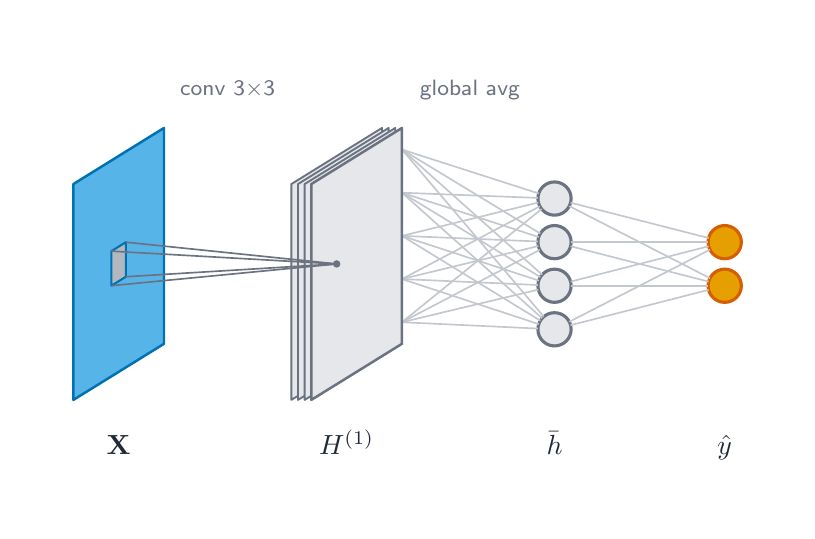
\begin{tikzpicture}[x=0.75pt, y=-0.75pt]
  \tikzset{
    xm hidden/.style={circle, minimum size=12pt, inner sep=0, outer sep=0, fill=xm2, draw=xm3, line width=1.13pt},
    xm output/.style={circle, minimum size=12pt, inner sep=0, outer sep=0, fill=xm4, draw=xm5, line width=1.13pt},
    xm edge/.style={draw=xm6, line width=0.6pt},
    xm map input/.style={fill=xm7, draw=xm8, line width=0.9pt, line join=round},
    xm map hidden back/.style={fill=xm2, draw=xm3, line width=0.68pt, line join=round},
    xm map hidden/.style={fill=xm2, draw=xm3, line width=0.9pt, line join=round},
    xm window/.style={fill=xm9, draw=xm8, line width=0.75pt, line join=round},
    xm ray/.style={draw=xm3, line width=0.6pt},
    xm ray end/.style={fill=xm3},
    xm name xm10/.style={text=xm10, inner sep=0, font=\sffamily\fontsize{9.75}{11.7}\selectfont},
    xm op xm3/.style={text=xm3, inner sep=0, font=\sffamily\fontsize{8.25}{9.9}\selectfont},
  }
  \fill[xm1] (0,0) rectangle (365.83,232.78);
  % Neurons
  \node[xm hidden] (n-2-0) at (253.83,82.33) {};
  \node[xm hidden] (n-2-1) at (253.83,103.33) {};
  \node[xm hidden] (n-2-2) at (253.83,124.33) {};
  \node[xm hidden] (n-2-3) at (253.83,145.33) {};
  \node[xm output] (n-3-0) at (335.83,103.33) {};
  \node[xm output] (n-3-1) at (335.83,124.33) {};
  % Connections 1
  \draw[xm edge] (180.32,58.71) -- (n-2-0);
  \draw[xm edge] (180.32,58.71) -- (n-2-1);
  \draw[xm edge] (180.32,58.71) -- (n-2-2);
  \draw[xm edge] (180.32,58.71) -- (n-2-3);
  \draw[xm edge] (180.32,79.51) -- (n-2-0);
  \draw[xm edge] (180.32,79.51) -- (n-2-1);
  \draw[xm edge] (180.32,79.51) -- (n-2-2);
  \draw[xm edge] (180.32,79.51) -- (n-2-3);
  \draw[xm edge] (180.32,100.31) -- (n-2-0);
  \draw[xm edge] (180.32,100.31) -- (n-2-1);
  \draw[xm edge] (180.32,100.31) -- (n-2-2);
  \draw[xm edge] (180.32,100.31) -- (n-2-3);
  \draw[xm edge] (180.32,121.11) -- (n-2-0);
  \draw[xm edge] (180.32,121.11) -- (n-2-1);
  \draw[xm edge] (180.32,121.11) -- (n-2-2);
  \draw[xm edge] (180.32,121.11) -- (n-2-3);
  \draw[xm edge] (180.32,141.91) -- (n-2-0);
  \draw[xm edge] (180.32,141.91) -- (n-2-1);
  \draw[xm edge] (180.32,141.91) -- (n-2-2);
  \draw[xm edge] (180.32,141.91) -- (n-2-3);
  % Connections 2
  \draw[xm edge] (n-2-0) -- (n-3-0);
  \draw[xm edge] (n-2-0) -- (n-3-1);
  \draw[xm edge] (n-2-1) -- (n-3-0);
  \draw[xm edge] (n-2-1) -- (n-3-1);
  \draw[xm edge] (n-2-2) -- (n-3-0);
  \draw[xm edge] (n-2-2) -- (n-3-1);
  \draw[xm edge] (n-2-3) -- (n-3-0);
  \draw[xm edge] (n-2-3) -- (n-3-1);
  % Layers
  \draw[xm map input] (22,75.35) -- (65.68,48.31) -- (65.68,152.31) -- (22,179.35) -- cycle;
  \draw[xm map hidden back] (127.04,75.35) -- (170.72,48.31) -- (170.72,152.31) -- (127.04,179.35) -- cycle;
  \draw[xm map hidden back] (130.24,75.35) -- (173.92,48.31) -- (173.92,152.31) -- (130.24,179.35) -- cycle;
  \draw[xm map hidden back] (133.44,75.35) -- (177.12,48.31) -- (177.12,152.31) -- (133.44,179.35) -- cycle;
  \draw[xm map hidden] (136.64,75.35) -- (180.32,48.31) -- (180.32,152.31) -- (136.64,179.35) -- cycle;
  \draw[xm window] (40.35,107.67) -- (47.33,103.35) -- (47.33,119.99) -- (40.35,124.31) -- cycle;
  \draw[xm ray] (40.35,107.67) -- (148.88,113.83);
  \draw[xm ray] (47.33,103.35) -- (148.88,113.83);
  \draw[xm ray] (47.33,119.99) -- (148.88,113.83);
  \draw[xm ray] (40.35,124.31) -- (148.88,113.83);
  \fill[xm ray end] (148.88,113.83) circle[radius=1.8];
  % Labels
  \node[xm name xm10, anchor=base] at (43.84,205.65) {$\mathbf{X}$};
  \node[xm op xm3, anchor=base] at (96.36,32.66) {conv 3\ensuremath{\times}3};
  \node[xm name xm10, anchor=base] at (153.68,205.65) {$H^{(1)}$};
  \node[xm op xm3, anchor=base] at (213.08,32.66) {global avg};
  \node[xm name xm10, anchor=base] at (253.83,205.65) {$\bar{h}$};
  \node[xm name xm10, anchor=base] at (335.83,205.65) {$\hat{y}$};
\end{tikzpicture}
\end{document}
